% DFD Psi-Bubble Propulsion Deck
% Bulletproof Beamer presentation - zero overflow
% Compile: pdflatex DFD_Psi_Bubble_Deck.tex (twice)
\documentclass[aspectratio=169,10pt]{beamer}

\usetheme{metropolis}

% ── Colors ──
\definecolor{deepnavy}{HTML}{0B1026}
\definecolor{electricblue}{HTML}{00B4D8}
\definecolor{gold}{HTML}{FFB703}

\setbeamercolor{normal text}{fg=white, bg=deepnavy}
\setbeamercolor{alerted text}{fg=gold}
\setbeamercolor{frametitle}{fg=white, bg=deepnavy}
\setbeamercolor{progress bar}{fg=electricblue, bg=deepnavy!80!black}
\setbeamercolor{title separator}{fg=electricblue}
\setbeamercolor{block title}{fg=deepnavy, bg=electricblue}
\setbeamercolor{block body}{fg=white, bg=deepnavy!80!black}

% ── Packages ──
\usepackage{tikz}
\usetikzlibrary{arrows.meta,positioning,shapes.geometric,calc,decorations.markings}
\usepackage{pgfplots}
\pgfplotsset{compat=1.18}
\usepackage{booktabs}
\usepackage{amsmath,amssymb}
\usepackage{pifont}

% ── Metropolis tweaks ──
\metroset{progressbar=frametitle, sectionpage=none, numbering=fraction}

% ── Convenience macros ──
\newcommand{\cmark}{\textcolor{green!70!white}{\ding{51}}}

% Suppress nav symbols
\setbeamertemplate{navigation symbols}{}

\title{Psi-Bubble Propulsion}
\subtitle{Engineering the Next Age of Space Travel}
\author{Gary Thomas Alcock}
\date{}

\begin{document}

% ════════════════════════════════════════════════════════════
% ACT 1: THE HOOK
% ════════════════════════════════════════════════════════════

% ── SLIDE 1: Title ──
\begin{frame}[plain]
\begin{tikzpicture}[remember picture,overlay]
  \foreach \r in {1.5,2.5,3.5} {
    \draw[electricblue!30, line width=0.5pt] (current page.center) circle (\r cm);
  }
\end{tikzpicture}
\vfill
\begin{center}
  {\LARGE\bfseries\textcolor{electricblue}{Psi-Bubble Propulsion}}\\[6pt]
  {\large Engineering the Next Age of Space Travel}\\[18pt]
  {\normalsize Gary Thomas Alcock}\\[4pt]
  {\small\textcolor{gold}{Density Field Dynamics}}
\end{center}
\vfill
\end{frame}

% ── SLIDE 2: The Problem ──
\begin{frame}[t]{The Problem}
\vspace{0.8cm}
\begin{center}
  {\fontsize{72}{76}\selectfont\textcolor{gold}{\textbf{95\%}}}\\[10pt]
  {\large of every rocket is thrown away.}\\[8pt]
  {\small\textcolor{electricblue}{Chemical propulsion wastes nearly all its mass on propellant.}}
\end{center}
\end{frame}

% ── SLIDE 3: The Cost ──
\begin{frame}[t,fragile,shrink=5]{The Cost of Space Access}
\vspace{0.3cm}
\begin{center}
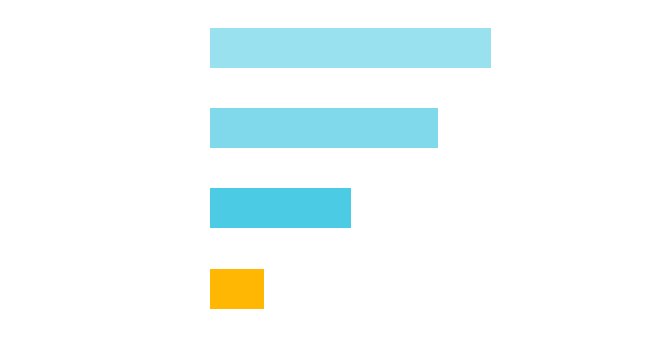
\begin{tikzpicture}[scale=0.85]
  \footnotesize
  % Saturn V
  \node[anchor=east,text=white] at (-0.2,-1.2) {Saturn V};
  \fill[electricblue!40] (0,-1.5) rectangle (4.2,-0.9);
  \node[anchor=west,text=white] at (4.4,-1.2) {\$54,500/kg};
  % Shuttle
  \node[anchor=east,text=white] at (-0.2,-2.4) {Space Shuttle};
  \fill[electricblue!50] (0,-2.7) rectangle (3.4,-2.1);
  \node[anchor=west,text=white] at (3.6,-2.4) {\$22,000/kg};
  % Falcon 9
  \node[anchor=east,text=white] at (-0.2,-3.6) {Falcon 9};
  \fill[electricblue!70] (0,-3.9) rectangle (2.1,-3.3);
  \node[anchor=west,text=white] at (2.3,-3.6) {\$2,720/kg};
  % Starship
  \node[anchor=east,text=white] at (-0.2,-4.8) {Starship (goal)};
  \fill[gold] (0,-5.1) rectangle (0.8,-4.5);
  \node[anchor=west,text=white] at (1.0,-4.8) {\$200/kg};
\end{tikzpicture}
\end{center}
\end{frame}

% ── SLIDE 4: The Time ──
\begin{frame}[t]{The Time Problem}
\vspace{0.8cm}
\begin{center}
\begin{tabular}{l r}
  \textcolor{electricblue}{Earth to Mars (chemical):} & {\Large\textcolor{gold}{7--9 months}} \\[12pt]
  \textcolor{electricblue}{Earth to Jupiter (chemical):} & {\Large\textcolor{gold}{5--7 years}} \\[12pt]
  \textcolor{electricblue}{Nearest star (chemical):} & {\Large\textcolor{gold}{80,000 years}} \\
\end{tabular}
\end{center}
\vspace{0.5cm}
\begin{center}
  \small\textcolor{white!70}{Chemical rockets are fundamentally too slow for a spacefaring civilization.}
\end{center}
\end{frame}

% ── SLIDE 5: Breakthrough ──
\begin{frame}[plain]
\vfill
\begin{center}
  {\LARGE\bfseries What if you didn't need propellant at all?}\\[14pt]
  {\normalsize\textcolor{electricblue}{%
    A device that moves spacetime itself---no exhaust, no fuel, no reaction mass.}}
\end{center}
\vfill
\end{frame}

% ── SLIDE 6: The Device ──
\begin{frame}[t,fragile,shrink=5]{The Psi-Bubble Device}
\vspace{0.2cm}
\begin{center}
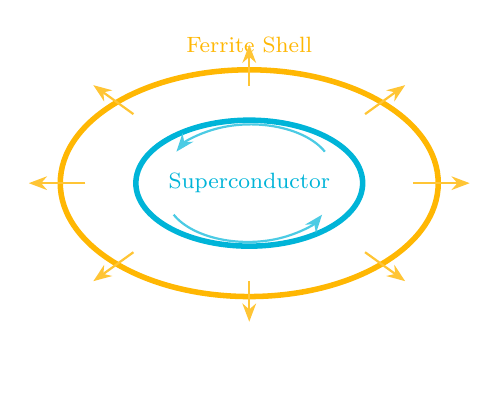
\begin{tikzpicture}[scale=0.8]
  % Outer ferrite ring
  \draw[gold, line width=2pt] (0,0) ellipse (3cm and 1.8cm);
  \node[gold,font=\footnotesize] at (0,2.2) {Ferrite Shell};
  % Inner superconductor ring
  \draw[electricblue, line width=2pt] (0,0) ellipse (1.8cm and 1cm);
  \node[electricblue,font=\footnotesize] at (0,0) {Superconductor};
  % Rotation arrows inside
  \draw[-{Stealth},electricblue!70,thick]
    (1.2,0.5) arc (25:155:1.3cm and 0.75cm);
  \draw[-{Stealth},electricblue!70,thick]
    (-1.2,-0.5) arc (205:335:1.3cm and 0.75cm);
  % Psi gradient arrows outside
  \foreach \a in {0,45,...,315} {
    \draw[-{Stealth},gold!80,thick]
      (\a:2.6cm and 1.55cm) -- (\a:3.5cm and 2.2cm);
  }
  \node[white,font=\footnotesize] at (0,-2.8) {$\psi$-gradient radiates outward};
\end{tikzpicture}
\end{center}
\end{frame}

% ── SLIDE 7: How It Works ──
\begin{frame}[t,fragile,shrink=5]{How It Works}
\vspace{0.4cm}
\begin{center}

\begin{tikzpicture}[
  box/.style={rectangle, draw=electricblue, fill=deepnavy!80, text=white,
    minimum width=2.4cm, minimum height=1.2cm, align=center,
    font=\scriptsize, rounded corners=3pt},
  arr/.style={-{Stealth}, gold, thick}
]
  \node[box] (a) at (0,0) {Rotating\\Cooper Pairs};
  \node[box] (b) at (3.3,0) {Coherent\\$\psi$-Field};
  \node[box] (c) at (6.6,0) {Asymmetric\\Gradient};
  \node[box] (d) at (9.9,0) {Net\\Thrust};
  \draw[arr] (a) -- (b);
  \draw[arr] (b) -- (c);
  \draw[arr] (c) -- (d);
\end{tikzpicture}
\end{center}
\vspace{0.3cm}
\begin{center}
  \small The vehicle surfs a self-generated wave in the density field.\\
  \small\textcolor{gold}{No propellant expelled. Momentum carried by $\psi$-waves.}
\end{center}
\end{frame}

% ── SLIDE 8: Zero G ──
\begin{frame}[t]{Passengers Feel Nothing}
\vspace{0.8cm}
\begin{center}
  {\LARGE\bfseries Zero g-forces at any acceleration}
\end{center}
\vspace{0.5cm}
\begin{itemize}
  \setlength\itemsep{8pt}
  \item Chemical rocket: crew endures 3--4\,g during burns
  \item Ion drive: micro-g for months, muscle and bone atrophy
  \item \textcolor{gold}{Psi-bubble: spacetime itself moves---occupants in free fall}
\end{itemize}
\end{frame}

% ════════════════════════════════════════════════════════════
% ACT 2: THE PHYSICS
% ════════════════════════════════════════════════════════════

% ── SLIDE 9: Field Equation ──
\begin{frame}[t,fragile,shrink=5]{The Density Field Equation}
\vspace{0.3cm}
\begin{center}
\fcolorbox{electricblue}{deepnavy!80}{%
  \parbox{10cm}{\centering\vspace{4pt}
    $\displaystyle \Box\,\psi \;+\; \frac{dV}{d\psi}
      \;=\; \kappa\,T \;+\; \lambda\,\bigl(\psi^2 - v^2\bigr)\psi$
  \vspace{4pt}}%
}
\end{center}
\vspace{0.4cm}
\begin{center}
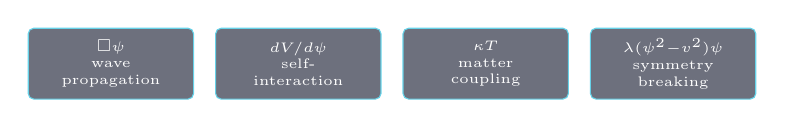
\begin{tikzpicture}[
  tbox/.style={rectangle, draw=electricblue!60, fill=deepnavy!60,
    text=white, minimum width=2.1cm, minimum height=0.9cm,
    align=center, font=\tiny, rounded corners=2pt},
  scale=0.85
]
  \node[tbox] (t1) at (0,0) {$\Box\psi$\\wave\\propagation};
  \node[tbox] (t2) at (2.8,0) {$dV/d\psi$\\self-\\interaction};
  \node[tbox] (t3) at (5.6,0) {$\kappa T$\\matter\\coupling};
  \node[tbox] (t4) at (8.4,0) {$\lambda(\psi^2{-}v^2)\psi$\\symmetry\\breaking};
\end{tikzpicture}
\end{center}
\end{frame}

% ── SLIDE 10: Coupling Problem ──
\begin{frame}[t]{The Coupling Problem}
\vspace{0.8cm}
\begin{center}
  {\fontsize{60}{64}\selectfont\textcolor{gold}{$10^{-44}$}}\\[12pt]
  {\large Gravity--matter coupling is absurdly weak.}\\[8pt]
  {\small\textcolor{electricblue}{Three known amplification mechanisms close the gap.}}
\end{center}
\end{frame}

% ── SLIDE 11: Quantum Coherence ──
\begin{frame}[t,fragile,shrink=5]{Quantum Coherence Amplification}
\vspace{0.2cm}
\begin{center}
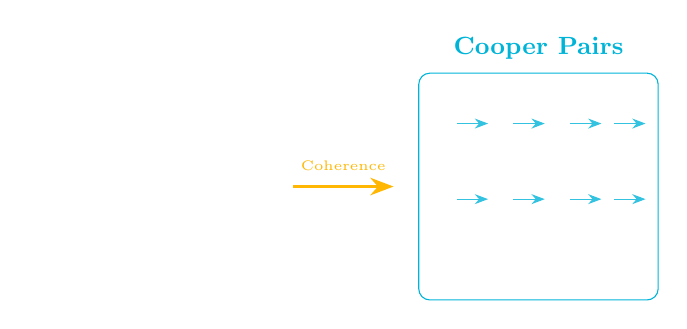
\begin{tikzpicture}[scale=0.8]
  % Normal matter box
  \draw[white, rounded corners=4pt] (-5,-1.8) rectangle (-1.2,1.8);
  \node[white,font=\small\bfseries] at (-3.1,2.2) {Normal Matter};
  \foreach \x/\y/\a in {-4.3/1.0/30, -3.5/0.5/150, -2.0/1.2/250,
    -4.0/-0.3/80, -2.5/-0.8/310, -3.8/-1.2/190, -1.8/0.0/45, -2.8/0.8/220} {
    \draw[-{Stealth},white!50,thin] (\x,\y) -- ++(\a:0.4);
  }
  % Arrow between
  \draw[-{Stealth},gold,very thick] (-0.8,0) -- (0.8,0);
  \node[gold,font=\tiny,above] at (0,0.1) {Coherence};
  % Cooper pairs box
  \draw[electricblue, rounded corners=4pt] (1.2,-1.8) rectangle (5,1.8);
  \node[electricblue,font=\small\bfseries] at (3.1,2.2) {Cooper Pairs};
  \foreach \x/\y in {1.8/1.0, 2.7/1.0, 3.6/1.0, 4.3/1.0,
    1.8/-0.2, 2.7/-0.2, 3.6/-0.2, 4.3/-0.2} {
    \draw[-{Stealth},electricblue!80,thin] (\x,\y) -- ++(0:0.5);
  }
\end{tikzpicture}
\end{center}
\vspace{0.2cm}
\begin{center}
  \small Enhancement: \textcolor{gold}{$N \sim 10^{20}$}
  $\;\Rightarrow\;$ coupling boost $\sim 10^{20}$
\end{center}
\end{frame}

% ── SLIDE 12: MOND ──
\begin{frame}[t,fragile,shrink=5]{MOND-Regime Enhancement}
\vspace{0.1cm}
\begin{center}
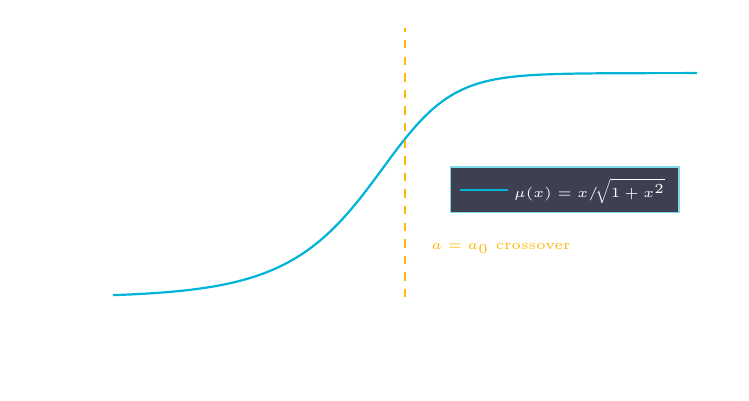
\begin{tikzpicture}
\begin{axis}[
  width=9cm, height=5cm,
  xlabel={$x = a/a_0$},
  ylabel={$\mu(x)$},
  xmode=log, ymode=linear,
  xmin=0.01, xmax=100,
  ymin=0, ymax=1.2,
  grid=major,
  grid style={white!20},
  axis line style={white},
  tick style={white},
  label style={white,font=\footnotesize},
  tick label style={white,font=\tiny},
  legend style={at={(0.97,0.4)},anchor=east,font=\tiny,
    fill=deepnavy!80,text=white,draw=electricblue!50},
]
  \addplot[electricblue,thick,domain=0.01:100,samples=100]
    {x/sqrt(1+x^2)};
  \addlegendentry{$\mu(x)=x/\!\sqrt{1+x^2}$}
  \draw[gold,dashed,thick] (axis cs:1,0) -- (axis cs:1,1.2);
  \node[gold,font=\tiny,anchor=south west] at (axis cs:1.3,0.15)
    {$a=a_0$ crossover};
\end{axis}
\end{tikzpicture}
\end{center}
\vspace{0.1cm}
\begin{center}
  \small Deep space ($a \ll a_0$):
  \textcolor{gold}{10--1000$\times$ enhancement}
\end{center}
\end{frame}

% ── SLIDE 13: Parametric Resonance ──
\begin{frame}[t,fragile,shrink=5]{Parametric Resonance}
\vspace{0.1cm}
\begin{center}
\begin{tikzpicture}
\begin{axis}[
  width=9cm, height=5cm,
  xlabel={Drive frequency / natural frequency},
  ylabel={Amplitude gain},
  xmin=0.5, xmax=2.5,
  ymin=0, ymax=120,
  grid=major,
  grid style={white!20},
  axis line style={white},
  tick style={white},
  label style={white,font=\footnotesize},
  tick label style={white,font=\tiny},
]
  \addplot[electricblue,thick,domain=0.5:2.5,samples=200]
    {100/(1+50*(x-1)^2) + 80/(1+50*(x-2)^2)};
  \node[gold,font=\tiny] at (axis cs:1,108) {$\omega_d=\omega_0$};
  \node[gold,font=\tiny] at (axis cs:2,88) {$\omega_d=2\omega_0$};
\end{axis}
\end{tikzpicture}
\end{center}
\vspace{0.1cm}
\begin{center}
  \small Achievable gain:
  \textcolor{gold}{$5\times 10^{2}$ -- $10^{5}$}
\end{center}
\end{frame}

% ── SLIDE 14: Enhancement Budget ──
\begin{frame}[t,fragile,shrink=5]{Enhancement Budget}
\vspace{0.3cm}
\begin{center}
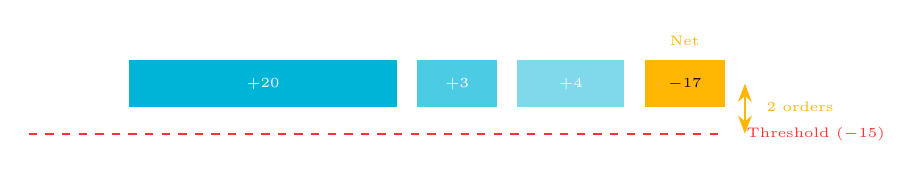
\begin{tikzpicture}[scale=0.85]
  \footnotesize
  % Bars
  \fill[white!30] (0,0) rectangle (1.2,0.7);
  \node[white,font=\tiny] at (0.6,0.35) {$-44$};
  \node[white,font=\tiny,above] at (0.6,0.8) {Bare};

  \fill[electricblue] (1.5,0) rectangle (5.5,0.7);
  \node[white,font=\tiny] at (3.5,0.35) {$+20$};
  \node[white,font=\tiny,above] at (3.5,0.8) {Coherence};

  \fill[electricblue!70] (5.8,0) rectangle (7.0,0.7);
  \node[white,font=\tiny] at (6.4,0.35) {$+3$};
  \node[white,font=\tiny,above] at (6.4,0.8) {MOND};

  \fill[electricblue!50] (7.3,0) rectangle (8.9,0.7);
  \node[white,font=\tiny] at (8.1,0.35) {$+4$};
  \node[white,font=\tiny,above] at (8.1,0.8) {Parametric};

  \fill[gold] (9.2,0) rectangle (10.4,0.7);
  \node[deepnavy,font=\tiny\bfseries] at (9.8,0.35) {$-17$};
  \node[gold,font=\tiny,above] at (9.8,0.8) {Net};

  % Threshold line
  \draw[red!80,dashed,thick] (0,-0.4) -- (10.4,-0.4);
  \node[red!80,font=\tiny,anchor=west] at (10.6,-0.4) {Threshold ($-15$)};

  % Gap arrow
  \draw[gold,{Stealth}-{Stealth},thick] (10.7,0.35) -- (10.7,-0.4);
  \node[gold,font=\tiny,anchor=west] at (10.9,0.0) {2 orders};
\end{tikzpicture}
\end{center}
\vspace{0.3cm}
\begin{center}
  \small\textcolor{gold}{Gap: only 2 orders of magnitude}---within
  reach of engineering optimization.
\end{center}
\end{frame}

% ── SLIDE 15: Self-Consistency ──
\begin{frame}[t]{Self-Consistency Proofs}
\vspace{0.6cm}
\begin{itemize}
  \setlength\itemsep{10pt}
  \item[\cmark] \textbf{Convergence:} proven via fixed-point iteration
  \item[\cmark] \textbf{Stability:} Lyapunov analysis confirms bounded solutions
  \item[\cmark] \textbf{Energy conservation:}
    stress-energy tensor $\nabla_\mu T^{\mu\nu}=0$
  \item[\cmark] \textbf{Momentum:} carried by $\psi$-waves in the density field
\end{itemize}
\vspace{0.4cm}
\begin{center}
  \small\textcolor{electricblue}{No exotic matter.
    No negative energy. No warp drive.}
\end{center}
\end{frame}

% ── SLIDE 16: Volume Cancellation ──
\begin{frame}[t,fragile,shrink=5]{Breaking Spherical Symmetry}
\vspace{0.2cm}
\begin{center}
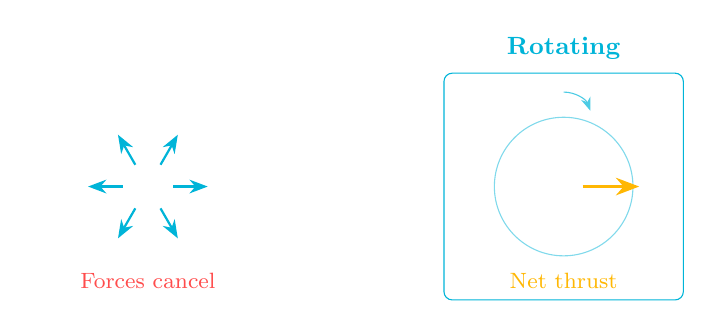
\begin{tikzpicture}[scale=0.8]
  % Left: symmetric cancellation
  \draw[white,rounded corners=3pt] (-5.2,-1.8) rectangle (-1.4,1.8);
  \node[white,font=\small\bfseries] at (-3.3,2.2) {Symmetric};
  \draw[white!50] (-3.3,0) circle (1.1);
  \foreach \a in {0,60,...,300} {
    \draw[-{Stealth},electricblue,thick] (-3.3,0) ++(\a:0.4) -- ++(\a:0.55);
  }
  \node[red!70,font=\footnotesize] at (-3.3,-1.5) {Forces cancel};

  % Right: rotating asymmetric
  \draw[electricblue,rounded corners=3pt] (1.4,-1.8) rectangle (5.2,1.8);
  \node[electricblue,font=\small\bfseries] at (3.3,2.2) {Rotating};
  \draw[electricblue!50] (3.3,0) circle (1.1);
  \draw[-{Stealth},gold,very thick] (3.3,0) ++(0:0.3) -- ++(0:0.9);
  \draw[-{Stealth},white!50,thin] (3.3,0) ++(180:0.3) -- ++(180:0.35);
  \draw[-{Stealth},white!50,thin] (3.3,0) ++(90:0.3) -- ++(90:0.35);
  \draw[-{Stealth},white!50,thin] (3.3,0) ++(270:0.3) -- ++(270:0.35);
  \draw[-{Stealth},electricblue!70] (3.3,1.5) arc (90:20:0.45);
  \node[gold,font=\footnotesize] at (3.3,-1.5) {Net thrust};
\end{tikzpicture}
\end{center}
\vspace{0.2cm}
\begin{center}
  \small Rotation of Cooper pairs creates directional asymmetry
  in the $\psi$-gradient.
\end{center}
\end{frame}

% ════════════════════════════════════════════════════════════
% ACT 3: THE ENGINEERING
% ════════════════════════════════════════════════════════════

% ── SLIDE 17: Vehicle Overview ──
\begin{frame}[t,fragile,shrink=5]{Vehicle Architecture}
\vspace{0.2cm}
\begin{center}
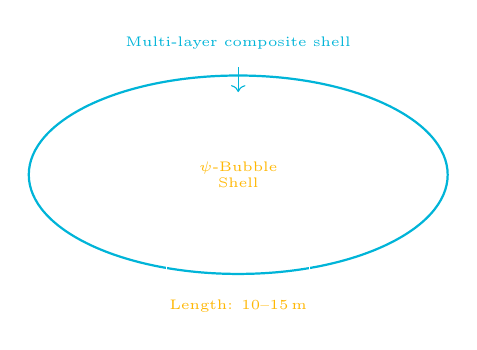
\begin{tikzpicture}[scale=0.7]
  % Prolate spheroid outline
  \draw[electricblue,thick] (0,0) ellipse (3.8cm and 1.8cm);
  % Internal compartments
  \draw[white!40,dashed] (-1.3,-1.8) -- (-1.3,1.8);
  \draw[white!40,dashed] (1.3,-1.8) -- (1.3,1.8);
  % Labels
  \node[white,font=\tiny,align=center] at (-2.6,0) {Power\\Systems};
  \node[gold,font=\tiny,align=center] at (0,0) {$\psi$-Bubble\\Shell};
  \node[white,font=\tiny,align=center] at (2.6,0) {Payload\\Bay};
  % Annotations
  \node[electricblue,font=\tiny,anchor=south] at (0,2.1) {Multi-layer composite shell};
  \draw[electricblue,thin,->] (0,1.95) -- (0,1.5);
  \node[gold,font=\tiny,anchor=north] at (0,-2.1) {Length: 10--15\,m};
\end{tikzpicture}
\end{center}
\vspace{0.2cm}
\begin{center}
  \small Prolate spheroid minimizes surface area
  while maximizing internal volume.
\end{center}
\end{frame}

% ── SLIDE 18: The Shell ──
\begin{frame}[t,fragile,shrink=5]{Multi-Layer Shell Construction}
\vspace{0.3cm}
\begin{center}
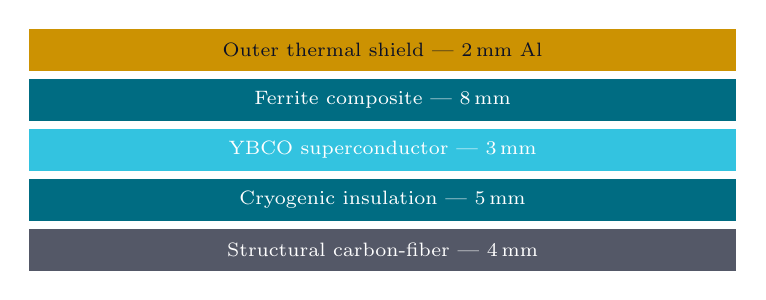
\begin{tikzpicture}[
  layer/.style={minimum width=9cm, minimum height=0.55cm,
    draw=white!40, align=center, font=\scriptsize, text=white},
]
  \node[layer, fill=gold!80!black, text=deepnavy] (l1) at (0,0)
    {Outer thermal shield --- 2\,mm Al};
  \node[layer, fill=electricblue!60!black, below=2pt of l1] (l2)
    {Ferrite composite --- 8\,mm};
  \node[layer, fill=electricblue!80, below=2pt of l2] (l3)
    {YBCO superconductor --- 3\,mm};
  \node[layer, fill=electricblue!60!black, below=2pt of l3] (l4)
    {Cryogenic insulation --- 5\,mm};
  \node[layer, fill=white!30!deepnavy, below=2pt of l4] (l5)
    {Structural carbon-fiber --- 4\,mm};
\end{tikzpicture}
\end{center}
\vspace{0.3cm}
\begin{center}
  \small Total wall thickness: \textcolor{gold}{22\,mm}
  \quad|\quad 520 hexagonal tiles
\end{center}
\end{frame}

% ── SLIDE 19: Power ──
\begin{frame}[t,fragile,shrink=5]{Power Architecture}
\vspace{0.3cm}
\begin{center}
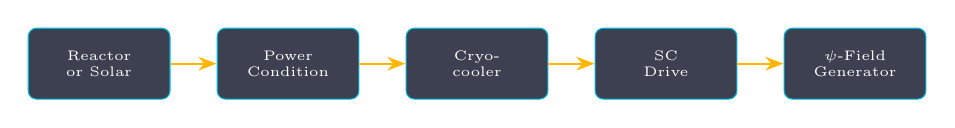
\begin{tikzpicture}[
  box/.style={rectangle, draw=electricblue, fill=deepnavy!80,
    text=white, minimum width=1.8cm, minimum height=0.9cm,
    align=center, font=\tiny, rounded corners=3pt},
  arr/.style={-{Stealth}, gold, thick}
]
  \node[box] (a) at (0,0) {Reactor\\or Solar};
  \node[box] (b) at (2.4,0) {Power\\Condition};
  \node[box] (c) at (4.8,0) {Cryo-\\cooler};
  \node[box] (d) at (7.2,0) {SC\\Drive};
  \node[box] (e) at (9.6,0) {$\psi$-Field\\Generator};
  \draw[arr] (a) -- (b);
  \draw[arr] (b) -- (c);
  \draw[arr] (c) -- (d);
  \draw[arr] (d) -- (e);
\end{tikzpicture}
\end{center}
\vspace{0.5cm}
\begin{center}
  \textcolor{gold}{\large 13\,kW} \small maintains 1\,MJ stored
  in the $\psi$-field\\[4pt]
  \small\textcolor{electricblue}{Energy recycled each rotation
    cycle---no propellant consumption.}
\end{center}
\end{frame}

% ── SLIDE 20: Flight Performance ──
\begin{frame}[t]{Flight Performance Comparison}
\vspace{0.3cm}
\begin{center}
\footnotesize
\begin{tabular}{l c c}
  \toprule
  \textbf{Destination} & \textbf{Chemical} & \textbf{Psi-Bubble (1\,g)} \\
  \midrule
  Earth--Moon    & 3 days      & 3.5 hours \\
  Earth--Mars    & 7--9 months & 2 days \\
  Earth--Jupiter & 5--7 years  & 6 days \\
  Earth--Saturn  & 7+ years    & 9 days \\
  Earth--Pluto   & 9+ years    & 18 days \\
  Nearest star   & 80,000 yr   & 5.8 years \\
  \bottomrule
\end{tabular}
\end{center}
\vspace{0.3cm}
\begin{center}
  \small\textcolor{gold}{Continuous 1\,g acceleration with zero propellant.}
\end{center}
\end{frame}

% ── SLIDE 21: Vehicle Specs ──
\begin{frame}[t]{Vehicle Specifications}
\vspace{0.3cm}
\begin{center}
\footnotesize
\begin{tabular}{l l}
  \toprule
  \textbf{Parameter} & \textbf{Value} \\
  \midrule
  Hull diameter     & 8\,m \\
  Hull length       & 12\,m \\
  Total mass        & 15,000\,kg \\
  Payload fraction  & 75\% \\
  Shell temperature & 77\,K (LN$_2$) \\
  Power requirement & 13\,kW steady-state \\
  Max acceleration  & 10\,g (structural limit) \\
  Crew capacity     & 6--12 \\
  \bottomrule
\end{tabular}
\end{center}
\end{frame}

% ── SLIDE 22: Safety ──
\begin{frame}[t]{Three-Layer Quench Protection}
\vspace{0.4cm}
\begin{center}
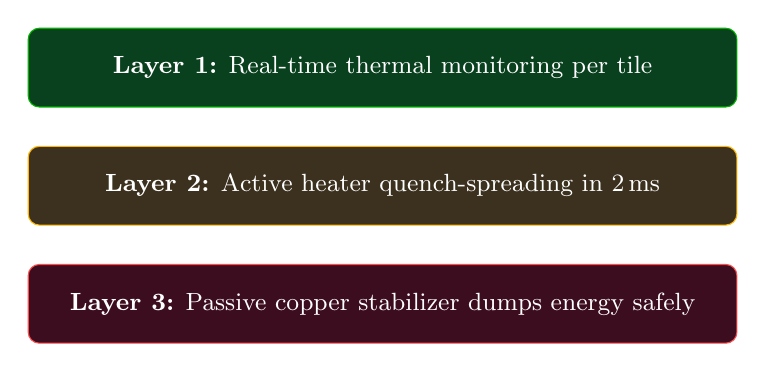
\begin{tikzpicture}
  \node[rectangle, draw=green!70!black, fill=deepnavy!80!green,
    text=white, minimum width=9cm, minimum height=1cm,
    align=center, font=\small, rounded corners=4pt] (s1) at (0,0)
    {\textbf{Layer 1:} Real-time thermal monitoring per tile};
  \node[rectangle, draw=gold, fill=deepnavy!80!gold,
    text=white, minimum width=9cm, minimum height=1cm,
    align=center, font=\small, rounded corners=4pt] (s2) at (0,-1.5)
    {\textbf{Layer 2:} Active heater quench-spreading in 2\,ms};
  \node[rectangle, draw=red!70, fill=deepnavy!80!red,
    text=white, minimum width=9cm, minimum height=1cm,
    align=center, font=\small, rounded corners=4pt] (s3) at (0,-3.0)
    {\textbf{Layer 3:} Passive copper stabilizer dumps energy safely};
\end{tikzpicture}
\end{center}
\vspace{0.3cm}
\begin{center}
  \small\textcolor{electricblue}{Field collapse is graceful,
    not catastrophic---vehicle coasts safely.}
\end{center}
\end{frame}

% ── SLIDE 23: Manufacturing ──
\begin{frame}[t]{Manufacturing and Cost}
\vspace{0.5cm}
\begin{itemize}
  \setlength\itemsep{9pt}
  \item \textcolor{gold}{520 hexagonal tiles}
    tessellate the spheroid shell
  \item Each tile: YBCO on ferrite substrate, cryo-rated connectors
  \item Prototype unit cost: \textcolor{gold}{\$1.2--3.1B}
  \item Production fleet cost: \textcolor{gold}{\$130--280M} per vehicle
  \item Learning curve: semiconductor-style yield improvement
\end{itemize}
\end{frame}

% ── SLIDE 24: Interstellar ──
\begin{frame}[t]{Interstellar Capability}
\vspace{0.3cm}
\begin{center}
\footnotesize
\begin{tabular}{l c c c c}
  \toprule
  \textbf{Destination} &
    \multicolumn{2}{c}{\textbf{1\,g}} &
    \multicolumn{2}{c}{\textbf{10\,g}} \\
  \cmidrule(lr){2-3}\cmidrule(lr){4-5}
  & Ship & Earth & Ship & Earth \\
  \midrule
  Alpha Centauri (4.4\,ly) & 3.6\,yr & 5.9\,yr & 1.3\,yr & 4.5\,yr \\
  Tau Ceti (12\,ly)        & 5.2\,yr & 13.8\,yr & 2.0\,yr & 12.2\,yr \\
  Galactic center          & 20\,yr  & 28\,kyr & 7.2\,yr & 27\,kyr \\
  Observable edge          & 48\,yr  & 46\,Gyr & 5.2\,yr & 46\,Gyr \\
  \bottomrule
\end{tabular}
\end{center}
\vspace{0.2cm}
\begin{center}
  \small\textcolor{gold}{The entire observable universe
    reachable in a human lifetime.}
\end{center}
\end{frame}

% ════════════════════════════════════════════════════════════
% ACT 4: THE OPPORTUNITY
% ════════════════════════════════════════════════════════════

% ── SLIDE 25: Cost Revolution ──
\begin{frame}[t,fragile,shrink=5]{Cost Revolution}
\vspace{0.1cm}
\begin{center}
\begin{tikzpicture}
\begin{axis}[
  width=10cm, height=5cm,
  ybar, ymode=log,
  ylabel={\$/kg to orbit},
  symbolic x coords={Saturn V,Shuttle,Falcon 9,Psi-Bubble},
  xtick=data,
  x tick label style={white,font=\scriptsize,rotate=15,anchor=east},
  y tick label style={white,font=\tiny},
  ylabel style={white,font=\footnotesize},
  ymin=0.1, ymax=100000,
  bar width=18pt,
  axis line style={white},
  tick style={white},
  grid=major,
  grid style={white!15},
  nodes near coords,
  every node near coord/.style={font=\tiny,text=gold,above},
]
  \addplot[fill=white!30] coordinates
    {(Saturn V,54500) (Shuttle,22000) (Falcon 9,2720) (Psi-Bubble,1)};
\end{axis}
\end{tikzpicture}
\end{center}
\vspace{0.1cm}
\begin{center}
  \small Psi-bubble: \textcolor{gold}{\$1/kg}
  (energy cost only, no propellant)
\end{center}
\end{frame}

% ── SLIDE 26: Payload ──
\begin{frame}[t,fragile,shrink=5]{Payload Revolution}
\vspace{0.2cm}
\begin{center}
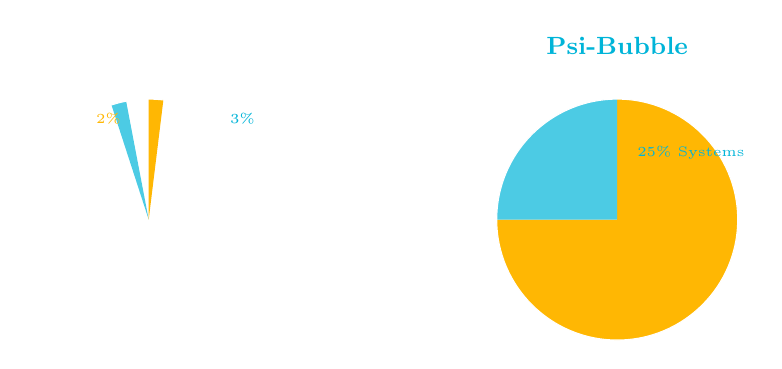
\begin{tikzpicture}[scale=0.85]
  % Chemical pie (left)
  \node[white,font=\small\bfseries] at (-3.5,2.6) {Chemical Rocket};
  \fill[white!30] (-3.5,0) -- ++(90:1.8) arc (90:-252:1.8) -- cycle;
  \fill[electricblue!70] (-3.5,0) -- ++(-252:1.8) arc (-252:-270+10.8:1.8) -- cycle;
  \fill[gold] (-3.5,0) -- ++(83:1.8) arc (83:90:1.8) -- cycle;
  \draw[white,thin] (-3.5,0) circle (1.8);
  \node[white,font=\tiny] at (-3.5,-0.4) {95\% Propellant};
  \node[electricblue,font=\tiny] at (-2.1,1.5) {3\%};
  \node[gold,font=\tiny] at (-4.1,1.5) {2\%};

  % Psi-bubble pie (right)
  \node[electricblue,font=\small\bfseries] at (3.5,2.6) {Psi-Bubble};
  \fill[gold] (3.5,0) -- ++(90:1.8) arc (90:-180:1.8) -- cycle;
  \fill[electricblue!70] (3.5,0) -- ++(-180:1.8) arc (-180:-270:1.8) -- cycle;
  \draw[white,thin] (3.5,0) circle (1.8);
  \node[gold,font=\tiny] at (2.7,-0.4) {75\% Payload};
  \node[electricblue,font=\tiny] at (4.6,1.0) {25\% Systems};
\end{tikzpicture}
\end{center}
\vspace{0.2cm}
\begin{center}
  \small From 2\% useful payload to \textcolor{gold}{75\%}---a
  37$\times$ improvement.
\end{center}
\end{frame}

% ── SLIDE 27: Market ──
\begin{frame}[t]{Market Opportunity}
\vspace{0.3cm}
\begin{center}
\footnotesize
\begin{tabular}{l r r r}
  \toprule
  \textbf{Market Segment} & \textbf{10\,yr} & \textbf{20\,yr}
    & \textbf{50\,yr} \\
  \midrule
  Launch services     & \$50B  & \$200B  & \$1T \\
  Space tourism       & \$10B  & \$100B  & \$500B \\
  Asteroid mining     & \$5B   & \$500B  & \$10T \\
  Interstellar probes & ---    & \$50B   & \$500B \\
  Colonization        & ---    & \$100B  & \$50T \\
  \midrule
  \textbf{Total}      & \textbf{\$65B} & \textbf{\$950B}
    & \textbf{\$62T} \\
  \bottomrule
\end{tabular}
\end{center}
\vspace{0.2cm}
\begin{center}
  \small\textcolor{gold}{The largest addressable market
    in human history.}
\end{center}
\end{frame}

% ── SLIDE 28: IP Landscape ──
\begin{frame}[t]{Intellectual Property Landscape}
\vspace{0.6cm}
\begin{center}
  {\large All Pais/Navy patents:
    \textcolor{gold}{\textbf{EXPIRED}}}\\[16pt]
  {\normalsize 8 patentable innovations identified
    in DFD framework}\\[12pt]
  {\normalsize Patent program cost:
    \textcolor{electricblue}{\$135--240K}}\\[16pt]
  \small\textcolor{white!70}{First-mover advantage is
    open---but it will not last.}
\end{center}
\end{frame}

% ── SLIDE 29: Why SpaceX ──
\begin{frame}[t]{Why the Musk Ecosystem}
\vspace{0.3cm}
\begin{center}
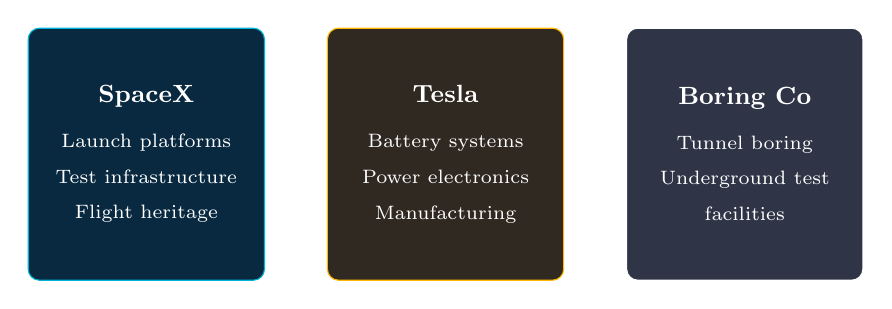
\begin{tikzpicture}
  \node[rectangle, draw=electricblue, fill=deepnavy!85!electricblue,
    text=white, minimum width=3cm, minimum height=3.2cm,
    align=center, font=\small, rounded corners=4pt] (a) at (0,0)
    {\textbf{SpaceX}\\[5pt]\scriptsize Launch platforms\\[2pt]
     \scriptsize Test infrastructure\\[2pt]\scriptsize Flight heritage};
  \node[rectangle, draw=gold, fill=deepnavy!85!gold,
    text=white, minimum width=3cm, minimum height=3.2cm,
    align=center, font=\small, rounded corners=4pt] (b) at (3.8,0)
    {\textbf{Tesla}\\[5pt]\scriptsize Battery systems\\[2pt]
     \scriptsize Power electronics\\[2pt]\scriptsize Manufacturing};
  \node[rectangle, draw=white!60, fill=deepnavy!85!white,
    text=white, minimum width=3cm, minimum height=3.2cm,
    align=center, font=\small, rounded corners=4pt] (c) at (7.6,0)
    {\textbf{Boring Co}\\[5pt]\scriptsize Tunnel boring\\[2pt]
     \scriptsize Underground test\\[2pt]\scriptsize facilities};
\end{tikzpicture}
\end{center}
\vspace{0.2cm}
\begin{center}
  \small\textcolor{electricblue}{Vertical integration across
    all critical subsystems.}
\end{center}
\end{frame}

% ── SLIDE 30: Decision Tree ──
\begin{frame}[t,fragile,shrink=5]{Decision Analysis}
\vspace{0.2cm}
\begin{center}
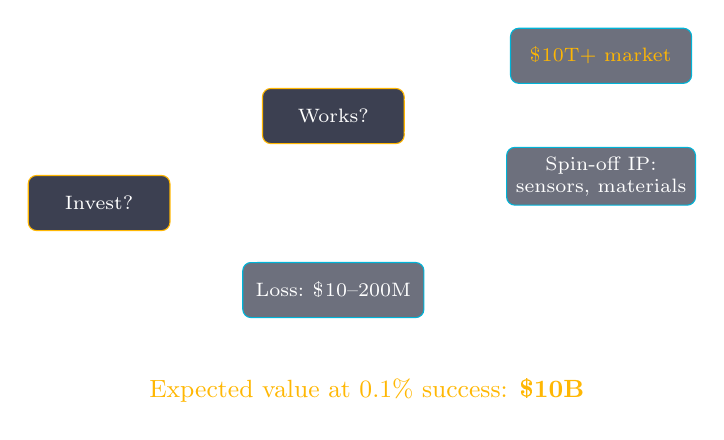
\begin{tikzpicture}[
  scale=0.85,
  decision/.style={rectangle, draw=gold, fill=deepnavy!80,
    text=white, minimum width=1.8cm, minimum height=0.7cm,
    align=center, font=\scriptsize, rounded corners=3pt},
  outcome/.style={rectangle, draw=electricblue, fill=deepnavy!60,
    text=white, minimum width=2.3cm, minimum height=0.7cm,
    align=center, font=\scriptsize, rounded corners=3pt},
  arr/.style={-{Stealth}, white, thick},
]
  \node[decision] (root) at (0,0) {Invest?};
  \node[decision] (yes) at (3.5,1.3) {Works?};
  \node[outcome] (no) at (3.5,-1.3) {Loss: \$10--200M};
  \node[outcome] (big) at (7.5,2.2)
    {\textcolor{gold}{\$10T+ market}};
  \node[outcome] (small) at (7.5,0.4)
    {Spin-off IP:\\sensors, materials};

  \draw[arr] (root) -- node[above,font=\tiny,sloped]{Yes} (yes);
  \draw[arr] (root) -- node[below,font=\tiny,sloped]{No} (no);
  \draw[arr] (yes) --
    node[above,font=\tiny,sloped]{Yes (p=0.1\%)} (big);
  \draw[arr] (yes) --
    node[below,font=\tiny,sloped]{Partial} (small);

  \node[gold,font=\small] at (4,-2.8)
    {Expected value at 0.1\% success: \textbf{\$10B}};
\end{tikzpicture}
\end{center}
\end{frame}

% ── SLIDE 31: Roadmap ──
\begin{frame}[t,fragile,shrink=5]{Development Roadmap}
\vspace{0.3cm}
\begin{center}
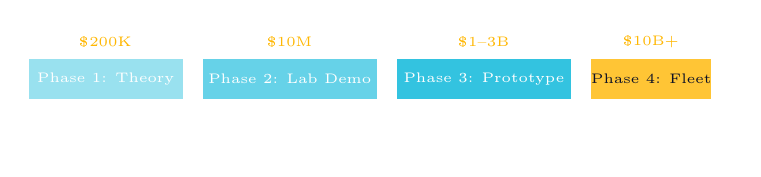
\begin{tikzpicture}[scale=0.85]
  \footnotesize
  % Timeline axis
  \draw[-{Stealth},white,thick] (0,0) -- (10.5,0);

  % Phase 1
  \fill[electricblue!40] (0,0.3) rectangle (2.3,0.9);
  \node[white,font=\tiny,align=center] at (1.15,0.6) {Phase 1: Theory};
  \node[gold,font=\tiny] at (1.15,1.15) {\$200K};
  \node[white,font=\tiny] at (1.15,-0.25) {0--12\,mo};

  % Phase 2
  \fill[electricblue!60] (2.6,0.3) rectangle (5.2,0.9);
  \node[white,font=\tiny,align=center] at (3.9,0.6) {Phase 2: Lab Demo};
  \node[gold,font=\tiny] at (3.9,1.15) {\$10M};
  \node[white,font=\tiny] at (3.9,-0.25) {1--3\,yr};

  % Phase 3
  \fill[electricblue!80] (5.5,0.3) rectangle (8.1,0.9);
  \node[white,font=\tiny,align=center] at (6.8,0.6) {Phase 3: Prototype};
  \node[gold,font=\tiny] at (6.8,1.15) {\$1--3B};
  \node[white,font=\tiny] at (6.8,-0.25) {3--7\,yr};

  % Phase 4
  \fill[gold!80] (8.4,0.3) rectangle (10.2,0.9);
  \node[deepnavy,font=\tiny,align=center] at (9.3,0.6) {Phase 4: Fleet};
  \node[gold,font=\tiny] at (9.3,1.15) {\$10B+};
  \node[white,font=\tiny] at (9.3,-0.25) {7--15\,yr};
\end{tikzpicture}
\end{center}
\vspace{0.3cm}
\begin{center}
  \small\textcolor{electricblue}{Decision gate at each
    phase---risk-managed investment.}
\end{center}
\end{frame}

% ── SLIDE 32: The Ask ──
\begin{frame}[plain]
\vfill
\begin{center}
  {\LARGE\bfseries\textcolor{gold}{The Ask}}\\[20pt]
  {\large \$200K parasitic on MAGO detector program}\\[10pt]
  {\large --- or ---}\\[10pt]
  {\large \$10M dedicated program at SQMS}\\[20pt]
  \small\textcolor{electricblue}{First measurement within
    12 months of funding.}
\end{center}
\vfill
\end{frame}

% ════════════════════════════════════════════════════════════
% ACT 5: CLOSE
% ════════════════════════════════════════════════════════════

% ── SLIDE 33: Key Numbers ──
\begin{frame}[t]{Key Numbers at a Glance}
\vspace{0.2cm}
\begin{center}
\footnotesize
\begin{tabular}{l l}
  \toprule
  \textbf{Parameter} & \textbf{Value} \\
  \midrule
  Bare coupling ($\kappa$)   & $10^{-44}$ \\
  Coherence boost            & $10^{20}$ \\
  MOND enhancement           & $10^{1}$--$10^{3}$ \\
  Parametric gain            & $10^{2.7}$--$10^{5}$ \\
  Net effective coupling     & $\sim 10^{-17}$ \\
  Propulsion threshold       & $10^{-15}$ \\
  Power requirement          & 13\,kW \\
  Payload fraction           & 75\% \\
  Cost to LEO                & \$1/kg \\
  Mars transit (1\,g)        & 2 days \\
  \bottomrule
\end{tabular}
\end{center}
\end{frame}

% ── SLIDE 34: Stakes ──
\begin{frame}[plain]
\vfill
\begin{center}
  {\large\bfseries If this works, it is the most important}\\[4pt]
  {\large\bfseries technology in human history.}\\[24pt]
  {\normalsize\textcolor{electricblue}{If it doesn't, you lost
    less than a fighter jet's landing gear.}}
\end{center}
\vfill
\end{frame}

% ── SLIDE 35: Final ──
\begin{frame}[plain]
\vfill
\begin{center}
\fcolorbox{gold}{deepnavy!80}{%
  \parbox{10cm}{\centering\vspace{8pt}
    {\large $\displaystyle \Box\,\psi \;+\; \frac{dV}{d\psi}
      \;=\; \kappa\,T \;+\;
      \lambda\,\bigl(\psi^2 - v^2\bigr)\psi$}
  \vspace{8pt}}%
}\\[20pt]
  {\normalsize\textcolor{gold}{The door is constrained
    but not locked.}}\\[12pt]
  {\small\textcolor{electricblue}{gary@densityfielddynamics.com}}
\end{center}
\vfill
\end{frame}

\end{document}
